\chapter{Introduction}

\begin{figure}[!h]
\centering
            \subfloat[t=0]{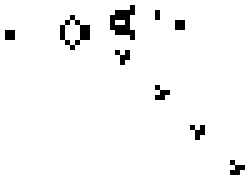
\includegraphics[width=.25\textwidth]{images/glider_gun/1.png}}\hfill
            \subfloat[t=10]{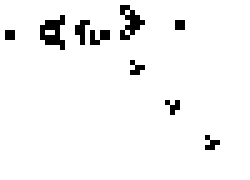
\includegraphics[width=.25\textwidth]{images/glider_gun/2.png}}\hfill
            \subfloat[t=20]{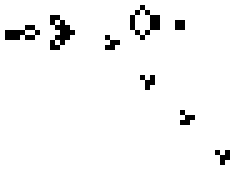
\includegraphics[width=.25\textwidth]{images/glider_gun/3.png}}\hfill
            \subfloat[t=30]{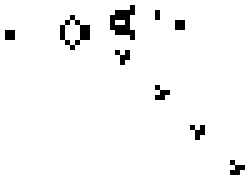
\includegraphics[width=.25\textwidth]{images/glider_gun/1.png}}\hfill
            \caption{Gosper's Glider Gun, the first known pattern to exhibit unbounded growth in Conway's Game of Life.\cite{hickerson}}
\label{fig:gospers-glider}
\end{figure}

\section{Motivation}
Predicting effects is easier than predicting causes. This is the crux of the Inverse Problem of Science. The causal opacity of time makes it easier to estimate observations from a parameterised model of the world than to deduce parameters from observations. Time eliminates information through the forces of selection and entropy. For instance, given knowledge of biological evolution, we may have strong hope of predicting where fossils of certain species lie but to build a rigorous taxomony based on fossils alone is insurmountably harder. A physical model of the universe may allow us to predict the subatomic particles ejected when two protons collide at high speed but building theories based on these collisions is difficult, especially when there are multiple equally valid explanations. Despite this, the pursuit of the Inverse Problem is critical to advancing scientific theory around a system's behaviour. Observations can only validate or falsify hypotheses but model prediction paves the way for novel scientific theories.\\

In this thesis, we tackle the inverse problem for cellular automata (CAs). These are simple yet powerful models of computation in which a discrete lattice of identical "cells" are simultaneously updated at regular time steps. The state of each cell depends exclusively on the state of the cells in a local neighbourhood around it in the previous time step. This localised interaction makes CAs a useful abstract representation for many physical and biological systems in the real world including tumor growth\cite{deutsch2021bio, reher2017cell}, urban land use\cite{white2000high}, and epidemics\cite{white2007modeling}. Much like these systems, CAs can exhibit chaos, nonlinear dynamics, and the emergence of complexity. As well as simulatory models, CAs are powerful computational engines due to ton a discrete lattice heir inherently parallel structure. This makes their study a useful endeavour in the field of distributed computation too\cite{tosic2005cellular}.\\

Top-down investigations into CA behaviour are vast and varied[CITE]. Mathematical analyses seek to classify CAs and prove general results about long-term behaviour from intrisic properties. In the natural and social sciences, CAs are designed to model real world systems. Both of these endeavours seek to analyse the behaviour of a CA from its structure, transition function, and initial conditions. In this thesis, we explore a bottom-up approach where we deduce the underlying properties of a CA by observing its behaviour. In particular, we utilise evolutionary algorithms to search across several classes of CA. Evolutionary algorithms (EAs) have long been held as effective tools for black-box optimisation problems. Grounded in the principles of Darwinian evolution, EAs traverse over a search space by performing selection, mutation, and crossover on a population of candidate solutions and discover increasingly strong solutions as the fitness of the population increases and selection pressure grows. Using EAs, we tackle multiple optimisation problems from the imitation of particular CA behaviour to the generation of desirable long-term states.\\

\section{Objectives}
We develop a system to discover cellular automata transition functions from observations. We focus on two classes of CA in particular. The first are binary outer-totalistic CA (see \ref{subsec:life-like-ga}) which are the discrete family of models in which Conway's infamous "Game of Life" CA belongs. For this reason, they are also called "life-like CA". The second are Gray-Scott models which simulate the behaviour of two diffusive chemicals. The density of each chemical in each cell is modelled as a lattice of real vector. Key aims of this project include:
\begin{enumerate}
    \item \textbf{Learning Full Rule Dynamics}\label{obj-1}\\
    Deduce the underlying transition rules behind life-like and Gray-Scott CA using genetic algorithms and evolutionary strategies.
    \item \textbf{Statistical Analysis of Rule Spaces}\\
    Assess which properties of cellular automata make them more or less predictable. Evaluate how this aligns with existing analyses in the literature.
    \item \textbf{Practical Application of Learning Pipeline}\\
    Use the tools from step~\ref{obj-1} to produce useful solutions to a real-world optimisation problems.
\end{enumerate}

\section{Contributions}
\begin{itemize}
    \item \textbf{Evolutionary Algorithm Toolkit}\\ A versatile toolkit that implements multiple evolutionary algorithms to train and optimise different classes of CA. We use this to successfully predict the update rule of life-like CA from observations on random initial conditions. We show that this can be extended to Gray-Scott models where we predict the parameters of diffusion-reaction equations from simulations of chemical reactions.
    \item \textbf{Cellular Automaton Simulator}\\ A system that can efficiently simulate discrete and continuous cellular automata. This allows various fitness functions to be implemented in the EA toolkit. This can also render snapshots of the CA directly during simulation which allows animations to be generated afterwards.
    \item \textbf{Procedural Maze Generator}\\ A CA-based maze generation program that uses the EA toolkit to produce difficult mazes. Mazes generated are guaranteed to have a solution and are optimised to exhibit characteristics preferred by users.
\end{itemize}

\section{Technical Challenges}

\begin{itemize}
    \item \textbf{Efficient Simulation}\\ Each evolutionary algorithm runs on large populations over multiple epochs and fitness is calculated by repeated simulation of individual CAs. This means that thousands of simulations need to be run for each experiment so the simulator must be implemented in an efficient manner. This is especially pertinent for the Gray-Scott simulator which uses numerical integration to approximate solutions for the continuous differential equations that underlie chemical interactions.
    \item \textbf{Avoiding Local Optima}\\ Evolutionary algorithms are very susceptible premature convergence. We tackle this by adjusting and testing a range of genetic operators, designing improved loss functions, and running large-scale simulations to produce heuristics that can assist with evolution.
    \item \textbf{Media Generation}\\ Effectively learning from experiments and iterating strategies required statistical summaries, images, and animations to be produced. These provide quantitative and qualitative feedback for later analysis. Converting numerical data into high-fidelity media was a key point of focus.
\end{itemize}
